
\documentclass{article}
\usepackage{fullpage}

%\setlength{\oddsidemargin}{0.25 in}
%\setlength{\evensidemargin}{-0.25 in}
%\setlength{\topmargin}{-0.6 in}
%\setlength{\textwidth}{6.5 in}
%\setlength{\textheight}{8.5 in}
%\setlength{\headsep}{0.75 in}
%\setlength{\parindent}{0 in}
%\setlength{\parskip}{0.1 in}



%%%% PACKAGES %%%%
\usepackage{algorithm,algorithmic}
\usepackage{amsfonts, amsmath, amsthm}
\usepackage{graphicx}
%for dotted lines inside matrices
\usepackage{arydshln}
\setlength{\dashlinedash}{.8pt} %
\setlength{\dashlinegap}{1.2pt}
%

%%%% ENVIRONMENTS %%%%
\newtheorem{definition}{Definition}[section]
\newtheorem{fact}{Fact}[section]
\newtheorem{claim}{Claim}[section]
\newtheorem{lemma}{Lemma}[section]
\newtheorem{remark}{Remark}[section]
\newtheorem{theorem}{Theorem}[section]
\newtheorem{proposition}{Proposition}[section]

%%%% COMMANDS %%%%
\newcommand{\E}{{\mathbb E}}
\newcommand{\Var}{{\operatorname{Var}}}
\newcommand{\var}{{\operatorname{Var}}}
\newcommand{\poly}{{\operatorname{poly}}}
\newcommand{\const}{{\operatorname{const}}}

\newcommand{\allones}{\mathbf{1}}
\newcommand{\abs}[1]{\left| #1 \right|}
\newcommand{\norm}[1]{\| #1 \|}
\newcommand{\eps}{\varepsilon}
\newcommand{\tab}{\hspace{.5cm}}
\newcommand{\R}{{\mathbb{R}}}
\newcommand{\Sph}{{\mathbb{S}}}
\newcommand{\N}{{\mathcal{N}}}


\newcommand{\lecture}[3]{
   %\pagestyle{myheadings}
   %\thispagestyle{plain}
   %\newpage
   %\setcounter{lecnum}{#1}
   %\setcounter{page}{1}
   \noindent
   \begin{center}
   \framebox{
      \vbox{\vspace{2mm}
    \hbox to 6.28in { {\bf 0368-3248-01-Algorithms in Data Mining
		\hfill Fall 2013} }
       \vspace{4mm}
       \hbox to 6.28in { {\Large \hfill Lecture #1: #2  \hfill} }
       \vspace{2mm}
       \hbox to 6.28in { {\it Lecturer: #3 \hfill}}% \hfill Scribes: #4} }
      \vspace{2mm}}
   }
   \end{center}
   \markboth{Lecture #1: #2}{Lecture #1: #2}
{\small
   {\bf Warning}: {\it This note may contain typos and other inaccuracies which are usually discussed during class. 
   Please do not cite this note as a reliable source. If you find mistakes, please inform me.}
   \vspace*{4mm}}
   \hrule
   \vspace{1cm}
}

%%%% COMMON DEFS %%%%
%\author{Edo Liberty \\ Class notes: Algorithms in Data mining}
\date{\nonumber}


\begin{document} %
\lecture{11}{Nearest Neighbor Search and the Curse of Dimensionality}{Edo Liberty}

Nearest neighbor search is a fundamental computational building block in computer vision, graphics, data mining, machine learning, and many other subfields.
As an example, consider a simple k-nearest-neighbor-classifier which, for each point predicts its class
by the a majority vote over its neighbors' classes. As simplistic as this classifier sounds, it actually performs 
very well in many scenarios. 

\begin{figure}[h!]
  \centering
  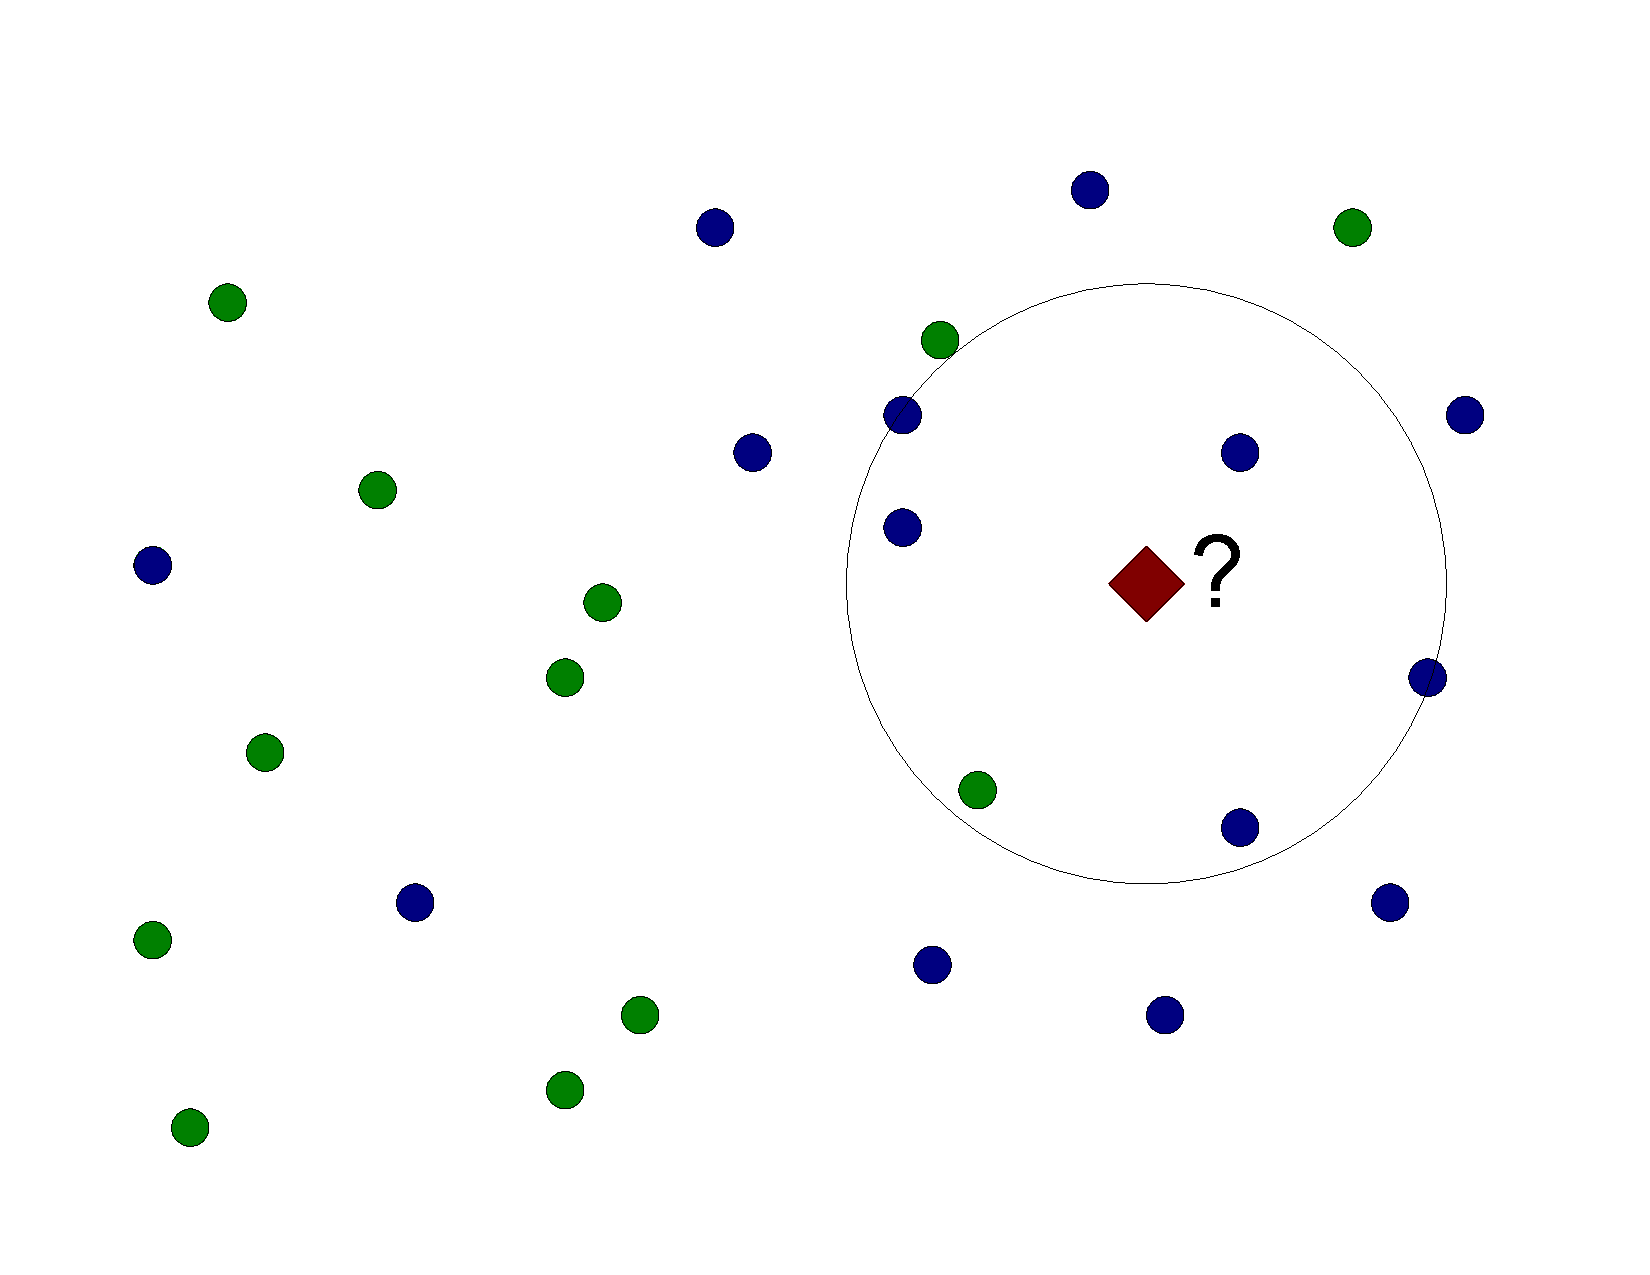
\includegraphics[width=0.6\textwidth]{11_images/knns_classifier.pdf}
  \caption{Illustration of the k-nearest neighbor classifier. The two classes are depicted by colors blue and green.
  The red rhombus will be tagged as being blue since most its neighbors are blue rather than green.}
\end{figure}

We could easily compute this by scanning the data points and finding those which minimize $\|q - x_i\|$.
But, of course, it would be significantly better if we could reduce the dependence on $n$, or in other words, avoid scanning the data for every query point.
One possible definition of the nearest neighbor problem is as follows:
\begin{definition}{\bf Nearest Neighbor Search:} Given a set of points $\{x_1,\ldots,x_n\} \in \R^{d}$ 
preprocess them into a data structure
$X$ of size $\poly(n,d)$ in time $\poly(n,d)$ such that nearest neighbor queries can
be performed in logarithmic time. In other words, given a search query point $q$ a radius $r$ and $X$ one can 
return all $x_i$ such the $||q - x_i || \le r$. The search for $x_i$ should require at most $\poly(d,\log(n))$ time.
\end{definition}


\section{kd-trees}
First, we shall review a well known an widely used algorithm for this problem which is called kd-trees \cite{Bentley75}.
The data structure holds the points in a tree. 
Each subtree contains all the points in an axis aligned bounding box (maybe infinite).
In each depth in the tree the bounding boxes are split along an axis (in a round robin order) at the median value of the points in the box.
Splitting stops when the number of points in the box is sufficiently small, say one. 


\begin{figure}[h!]
  \centering
  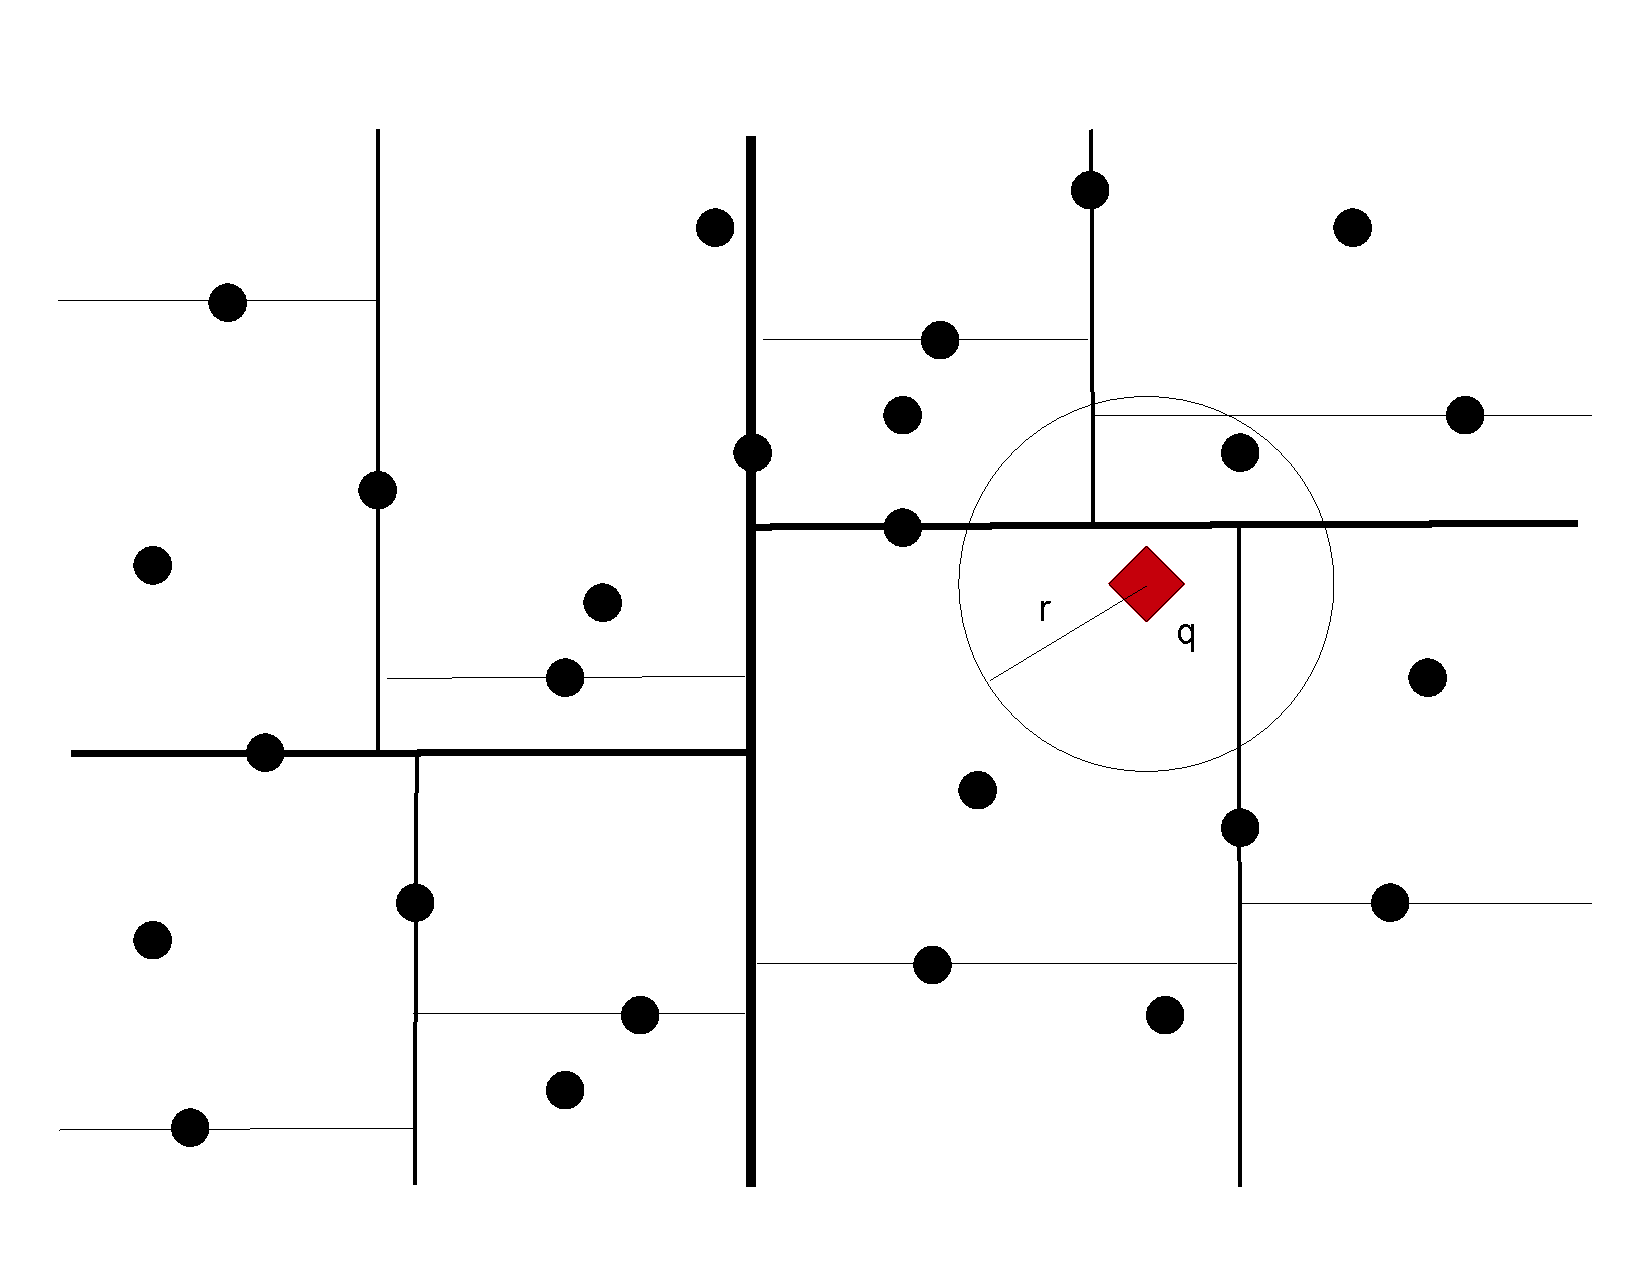
\includegraphics[width=0.6\textwidth]{11_images/nns.pdf}
  \caption{Illustration of space partition generated by the kd-tree algorithm in $\R^2$. 
  The width of the separating lines indicate the depth in the tree of the corresponding split.}
\end{figure}
It is quite simple to prove that inserting and deleting points requires $O(log(n))$ time.
Thus, the entire construction time is bounded by $O(n\log(n))$.

Searching however is quite a different matter.
Let us assume w.o.l.g.\ that all points are inside the unit cube. 
A harmless assumption because we can scale the entire data set by a constant factor.
Also, notice that each point in the date whose bounding box intersects the query sphere must be
examined. Moreover, examining each data point can generate at most $O(log(n))$ computations.
We will therefore only ask ourselves, how many point boxes have a non zero intersection with the query sphere.

To make this exercise simpler, consider a simpler case and a variation of kd-trees.
First, all $n$ data points are distributed uniformly and i.i.d. over $[0,1]^{d}$.
Also, the space partition splits every box exactly in the middle when the cut is
made along the axes in a round robin order.
Note that for such random data, our simple algorithm produces a very simple partition to the
one kd-tree would have generated since the median point is approximately also in the middle of the box.
(this holds as long as the number of points in a box is large enough)

Let's assume each box is split $t$ times (the depth of the tree is $t$). 
That means that each axis was split in half $t/d$ (assuming $t/d$ is an integer) times.
Therefore, the dimension of our box are $[2^{-t/d},2^{-t/d},\ldots,2^{-t/d}]$.
What is the probability that a (randomly located) ball of radius $r$ will hit this box?

\begin{figure}[h!]
  \centering
  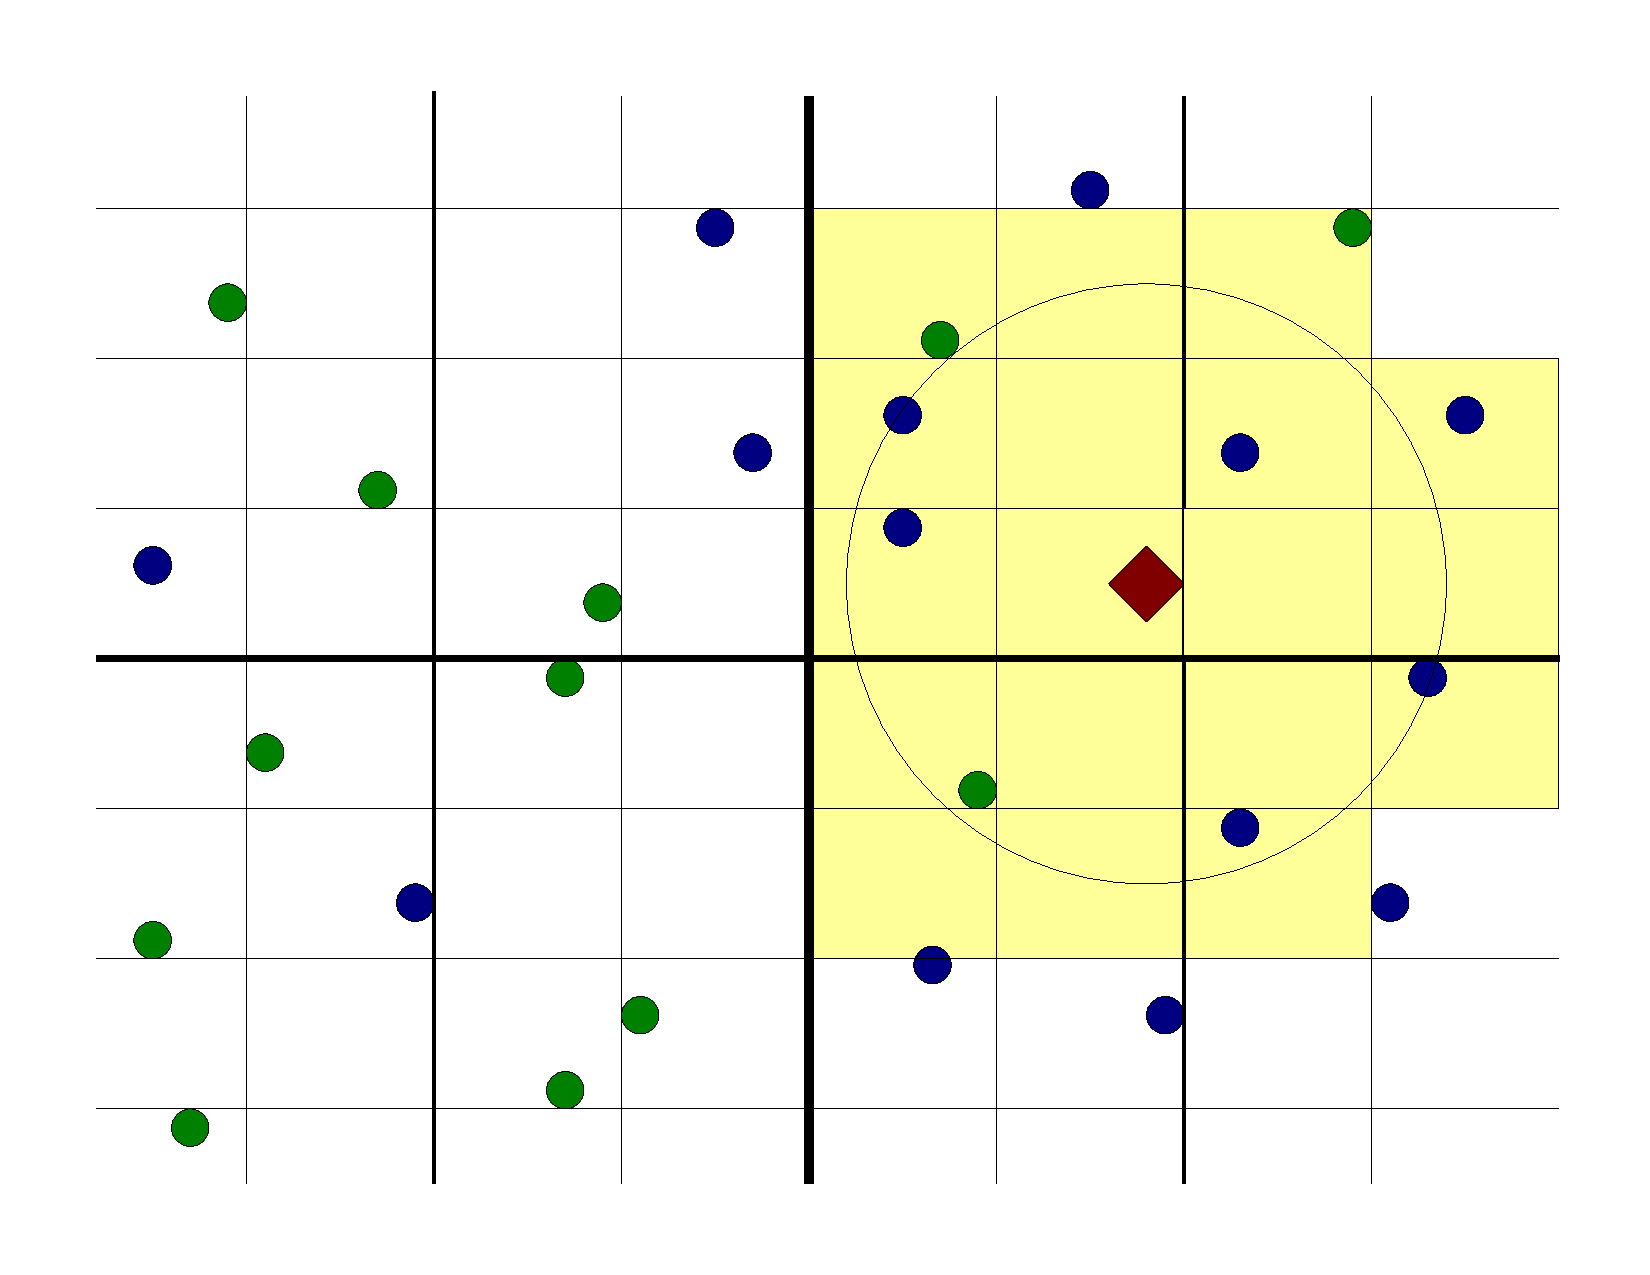
\includegraphics[width=0.6\textwidth]{11_images/nns_simple.pdf}
  \caption{Illustration of space partition generated by the kd-tree algorithm in $\R^2$. 
  The width of the separating lines indicate the depth in the tree of the corresponding split.}
\end{figure}


\begin{figure}[h!]
  \centering
  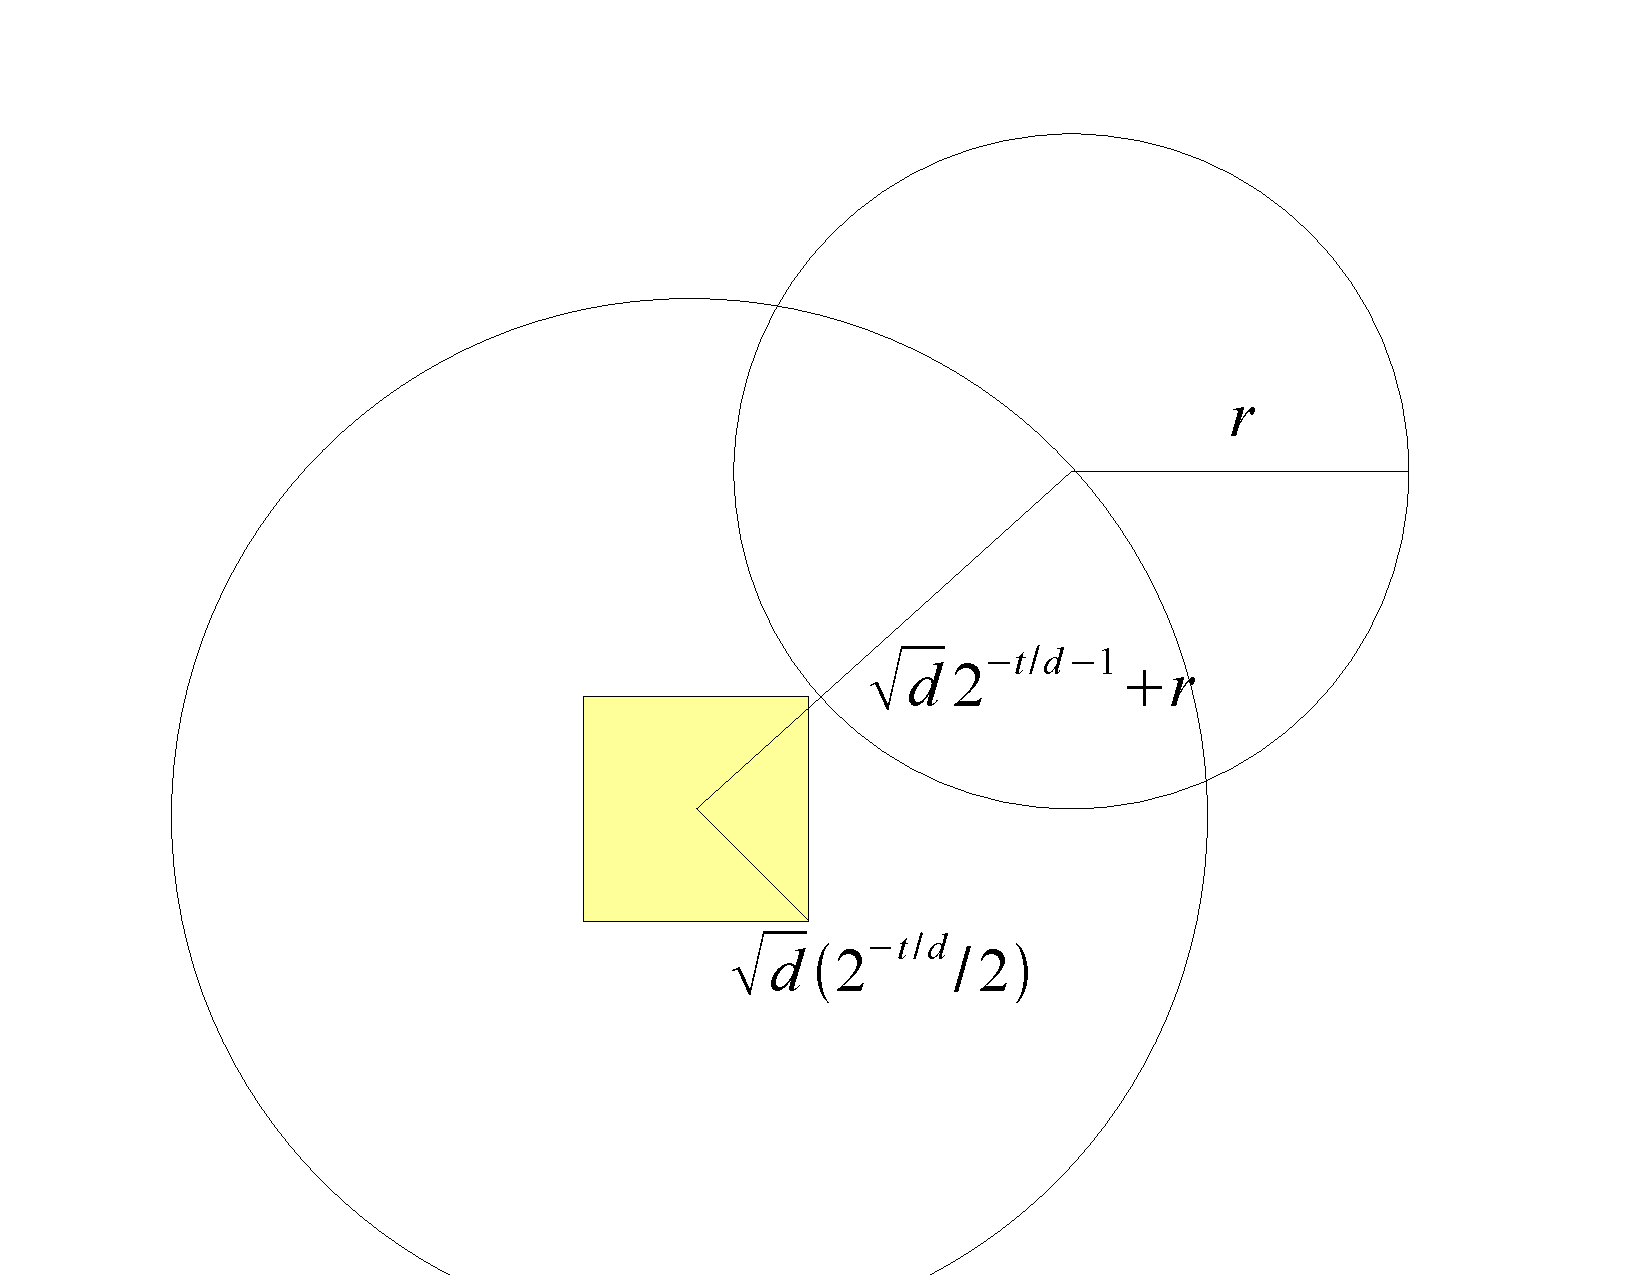
\includegraphics[width=0.6\textwidth]{11_images/radii.pdf}
  \caption{If the query point falls more than $\sqrt{d}2^{-t/d-1} + r$ away from the center of a 
  box it cannot be `hit'.}
\end{figure}

This probability that the box is ``hit" by a random query sphere 
is at most the volume of a sphere of radius $\sqrt{d}2^{-t/d-1} + r$ since 
if the query falls outside this ball it will not intersect the box. Assume, for now, that $\sqrt{d}2^{-t/d-1} \le r$ and
so the probability of this event is bounded by the volume of a ball of radius $2r$.
The volume of such a ball is $\pi^{d/2}(2r)^d/(d/2)!$ (assuming, for convenience, that $d$ is even).
The dependance on the radius is therefore $O(r^d)$. Thus, we can expect to inspect only a $O(r^d)$ fraction of the 
boxes (and thus points). Since $r\le 1$ this can be a significant speedup.

We saw that separating the space into boxes enabled us to search in it more efficiently.
We, however, made some heavy assumptions. One such is that $\sqrt{d}2^{-t/d-1} \le r$.
This assumption fails when the dimension grows. To see this, consider that $t \approx \log(n)$ 
to give boxes of volume roughly $1/n$. Requiring that $\sqrt{d}2^{-\log(n)/d} \le \sqrt{d}/2$ we get that $\log(n) \ge d$ or that $n$ must be
exponential in $d$, $n \ge 2^{d}$. Therefore, we only gain if the number of points in exponential in the dimension.
This is a result of the so called ``curse of dimensionality'' which is discussed next.

\section{Curse of dimensionality}
\subsection{kd-trees fail in high dimensions}
A prime example for the curse of dimensionality is that a random point in $[0,1]^d$ is likely to be far from any set of $n$ points in the unit cube.
Consider the distance between the query point $q$ and an input data vector $x$.
We want to show that $\|x_i-q\|^2 \in \Omega(d)$.

First, notice that $\Pr[|x(j)- q(j)| \ge 1/4] \ge 1/2$. The expected distance between $x$ and $q$ is at least $d/8$.
Since $q(j)$ are independently drown, we can apply the Chernoff bound and get that for all $n$ points in the data set
$\|x_i-q\|^2 \ge d/16$ if $d \ge \const\cdot\log(n)$.

Now, consider the kd-tree data structure and algorithm run on a random query.
If the radius of the ball around $q$ is less than $d/16$ the query is ``uninteresting'' since it is likely to return no results at all.
On the other hand, if the radius is greater than $d/16$ than the ball around $q$ will cross all the major partitions 
along one of the axis. That means that the algorithm will visit at least $2^d$ partitions.


\subsection{Volumes of balls and cubes}
Another interesting phenomenon that occurs in high dimensions in the fact that unit spheres 
are exponentially smaller (in volume) than their containing boxes.
Let us see this without using the explicit formulas for the volume of $d$ dimensional spheres.

To compute the volume of a unit sphere, we perform a thought experiment.
First, bound the sphere in a box (with sides of length $2$).
Then, pick a point in the box uniformly at random. What is the probability $p$ that
the point is also in the sphere? This is exactly the ratio between the volume of the ball and the box ($2^d$).
More accurately, $V = p2^d$ where $V$ is the volume of the sphere.

Now, we can bound $p$ from above. 
A uniformly random chosen point from the cube is a vector $x \in \R^d$ such that each coordinate $x(i)$
is chosen uniformly from $[-1,1]$. The event that $x$ is in the unit sphere is the event that $\|x\|^2 = \sum_{i=1}^{d}x(i)^2 \le 1$.
Let $z_i = x(i)^2$, and note that 
$\E[z(i)] = \int_{-1}^{1}\frac{1}{2}t^2 dt = 1/3$. Therefore, $\E[\|x\|^2] = d/3$. 
Also, 
\[
\var(z_i)  = \int_{-1}^{1}\frac{1}{2}t^4 dt  - (1/3)^2  = 1/5 - 1/9 \le 1/10
\]
so by Chernoff's inequality.
$p = \Pr[\sum_{i=1}^{d}x(i)^2 \le 1]  = \Pr[\sum_{i=1}^{d}(z_i -\E[z_i] ) \le 1-d/3] \le e^{-\frac{(d/3)^2}{4d/10}} \le e^{-d/4}$.
This concludes the observation that the fraction of the volume which is inside the sphere is 
exponentially small compared to the cube.
A counter intuitive way of viewing this is that almost the entire volume of the cube is concentrated at the ``corners".

\subsection{Orthogonallity of random vectors}

It turns out that two random vectors are also almost orthogonal.
We can see this in two ways.

First, we can see that the expected, dot product of any vector $x$ with a random vector $y$ is small.
It is trivial that $\E[\langle x,y \rangle] = 0$ since the distribution of $y$ is symmetric.
Moreover, $\E[\langle x,y \rangle^2] = 1/d$.
To see this, consider $y_1,y_2,\ldots,y_d$ where $y_1 = y$ and $y_2,\ldots,y_d$ complete $y$ to an orthogonal basis.
Clearly, the distribution of all $y_i$ are identical (but not independent)
$\E[\langle x,y \rangle^2] = \E[\langle x,y_1\rangle^2] = \E[\frac{1}{d}\sum_{i=1}^{d}\langle x,y_i\rangle^2] = \frac{1}{d}\|x\|^2 = \frac{1}{d}$.

It is not hard to show that in fact for any vector $x$, if $y$ is chosen uniformly at random from the unit sphere 
then $\Pr[ \langle x,y \rangle  \ge \frac{t}{\sqrt{d}}] \le e^{-t^2/2}$.
First, replace that uniform distribution over the unit sphere with an i.i.d. distribution of gaussians $y(i)\sim \N(0,\frac{1}{\sqrt{d}})$.
Note that $E[\|y\|^2] = 1$, moreover, from the sharp concentration of the $\chi^2$ distribution we know that $E[\|y\|^2] \approx 1$.
For convenience we will assume that $E[\|y\|^2] = 1$ and will ignore the small inaccuracy.
Moreover, due to the rotational invariance of the Gaussian distribution we have that any direction is equally likely and thus this
new distribution approximates the uniform distribution over the sphere.
Next, notice that due to the rotational invariance $\langle x,y \rangle \sim \N(0,\frac{\|x\|}{\sqrt{d}}) = \N(0,\frac{1}{\sqrt{d}})$.
Therefore, letting $Z \sim \N(0,1)$ we have $\Pr[ \langle x,y \rangle  \ge \frac{t}{\sqrt{d}}] = \Pr[Z \ge t] \le e^{-t^2/2}$.



\bibliographystyle{plain}
\bibliography{AlgorithmsInDataMining.bib}

\end{document}













%%%%%%%%
